%
% introduction.tex
%
% Copyright (C) 2021 by SpaceLab.
%
% EPS 2.0 Documentation
%
% This work is licensed under the Creative Commons Attribution-ShareAlike 4.0
% International License. To view a copy of this license,
% visit http://creativecommons.org/licenses/by-sa/4.0/.
%

%
% \brief Introduction chapter.
%
% \author Gabriel Mariano Marcelino <gabriel.mm8@gmail.com>
% \author Yan Castro de Azeredo <yan.ufsceel@gmail.com>
%
% \institution Universidade Federal de Santa Catarina (UFSC)
%
% \version 0.2.0
%
% \date 2021/03/16
%

\chapter{Introduction} \label{ch:introduction}

The EPS 2.0\nomenclature{\textbf{EPS}}{\textit{Electric Power System.}} is a PCB\nomenclature{\textbf{PCB}}{\textit{Printed Circuit Board.}} designed to harvest, store and distribute energy for a nanosatellite. It is one of the service modules developed for FloripaSat-2 CubeSat Mission \cite{floripasat2-doc}. The energy harvesting system is based on solar energy conversion through ten solar panels attached to the 2U CubeSat structure. The EPS 2.0 is designed to operate the solar panels at their maximum power point (MPPT)\nomenclature{\textbf{MPPT}}{\textit{Maximum Power Point Tracking.}}. The board is also responsible for measuring solar panels current, voltage and the temperature of the panels and batteries. The harvested solar energy is stored in the Battery Module 4C \cite{bat4c} connected to the EPS. The energy distribution is done by several integrated buck DC-DC converters. The full EPS system is composed of the solar panels, the EPS 2.0 PCB and the battery module. The module is capable to measure its power consumption and operate in a lower energy state if needed. A general view of the EPS 2.0 board can be seen in \autoref{fig:general-view}.

The module is a direct upgrade from the EPS of FloripaSat-1 \cite{eps-fsat}, which grants a flight heritage rating. The improvements focus on providing a cleaner and more generic implementation in comparison with the previous version, more reliability in software, and adaptations for the new mission requirements. All the project, source and documentation files are available freely on a GitHub repository \cite{eps2} under its respective licenses.

\begin{figure}[!ht]
    \begin{center}
        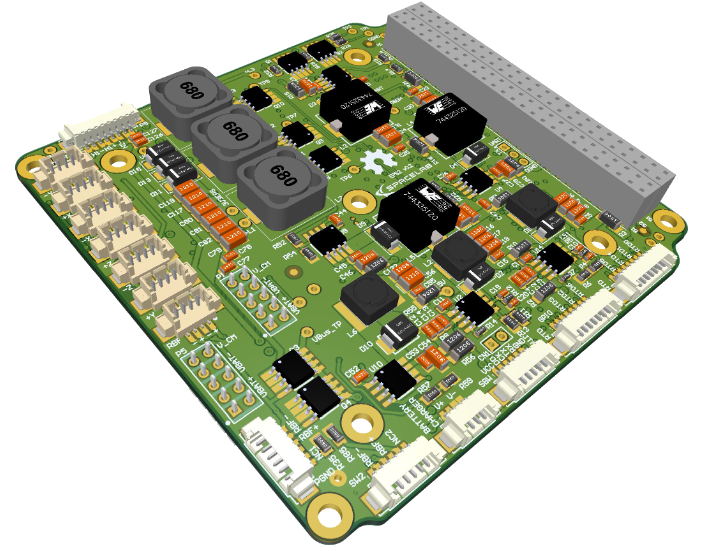
\includegraphics[width=0.55\textwidth]{figures/eps2-pcb-3d}
        \caption{3D view of the EPS 2.0 PCB.}
        \label{fig:general-view}
    \end{center}
\end{figure}